
\section{Regresija}

Ni polinomijalna interpolacija ni kubični splajn nisu dobri za aproksimaciju
vrijednosti koje nisu omeđene poznatim vrijednostima.
\begin{itemize}
    \item Kubični splajn ima manje oscilacije, no i dalje se pojavljuju značajne
    oscilacije i odstupanja na krajnjim segmentima.
    \item Interpolacijom se greške u mjerenim podacima "ugrađuju" u
    interpolacijsku funkciju.
\end{itemize}

Regresija je metoda određivanja funkcije koja blisko prati zadane podatke na
način gdje opisuje njihovo ponašanje uz \textbf{minimalno rasipanje izmjerenih
vrijednosti oko poznatih segmenata}. Dakle, neće davati vrijednosti jednake
izmjerenim podacima, nego njima \textbf{bliske vrijednosti}.

\textbf{Udaljenost} $d_i$ zadane točke $(x_i, y_i)$ od točke na grafu se mjeri
normom. Najčešći izbor je $\mathrm{L}_2$ norma oblika

$$
d_i=\sqrt{(x_i-x_i)^2+(y_i-f(x_i))^2}.
$$

Tako se kao "najbliža" funkcija smatra onom kod koje su te udaljenosti po svim
točkama najmanje. Budući da su $d_i\geq0, i\in[0,n]$, to znači da je
\textbf{najbliža funkcija} ona kod koje je suma $\sum_{i=0}^nd_i$ najmanja.
Traženje minimuma te sume može biti problematično pa se u praksi uvijek traži
minimum sume

\begin{equation}
    \label{sum_squares}
    \sum_{i=0}^nd_i^2
\end{equation}

koja daje jednake rezultate, ali ih je znatno lakše odrediti.

Minimiziranje sume kvadrata udaljenosti se smatra kriterijem kod metode
regresije pa se metoda regresije također naziva i \textbf{metodom najmanjih
kvadrata}.

Nemoguće je naći minimum sume \ref{sum_squares} na skupu svih mogućih funkcija.
Za zadane točke \textbf{prvo biramo model ili klasu funkcije} između kojih ćemo
tražiti onu koja minimizira sumu \ref{sum_squares}.

\subsection{Linearna regresija}

Najjednostavniji odabir je traženje funkcije na skupu svih pravaca $f(x) = a_0 +
a_1x$ i takvu regresiju zovemo \textbf{linearna regresija}. Tako problem
minimizacije \ref{sum_squares} svodimo na problem određivanja koeficijenata
$a_0$ i $a_1$ u sumi

$$
S = \sum_{i=0}^n(y_i - (a_0+a_1x_i))^2
$$

Dakle radi se o funkciji $S=S(a_0,a_1)$ s dvije varijable kojoj jednostavno
nalazimo minimum.

Prirodno, zadajemo uvjete za stacionarnu točku funkcije dvije varijable

$$
\partial_{a_0}S=0,\qquad\partial_{a_1}S=0.
$$

Nakon sređivanja uvjeti daju sustav dvije linearne jednadžbe

\begin{align*}
a_0(n+1)+a_1\sum_{i=0}^nx_i=&\sum_{i=0}^ny_i\\
a_0\sum_{i=0}^nx_i+a_1\sum_{i=0}^nx_i^2=&\sum_{i=0}^nx_iy_i
\end{align*}

za dvije nepoznanice $a_0$ i $a_1$.

Osim kod izuzetno nepovoljnog rasporeda točaka koji uistinu ne odgovara pravcu,
ovaj \textbf{sustav ima determinantu različitu od nule} te time i jedinstveno
rješenje, kada je broj točaka za koje ga rješavamo n$\geq2$. Budući da je
$S\geq0$, rješenje mora biti lokalni minimum te je time problem metode linearne
regresije u potpunosti riješen.

\begin{example}[uporaba metode najmanjih kvadrata]
    Podatke zadane tablicom aproksimirati linearnom funkcijom koristeći metodu
    najmanjih kvadrata.

    \center
    \begin{tabular}{r|c|c|c}
        $x$ & 0 & 1 & 3 \\
        \hline
        $y$ & 1 & 2 & 3
    \end{tabular}
\end{example}

\subsection{Kvadratna regresija}

U slučaju kvadratne funkcije oblika

$$
f(x) = a_0+a_1x+a_2x^2
$$

imamo sumu

$$
S = \sum_{i=0}^n(y_i - (a_0+a_1x+a_2x^2))^2
$$

te potrebno zadati uvjete stacionarne točke za funkciju s 3 varijable:

$$
\partial_{a_0}S=0,\qquad\partial_{a_1}S=0,\qquad\partial_{a_2}S=0.
$$

Sređivanjem dobivamo sustav koji određuje koeficijente funkcije:

\begin{align*}
    a_0(n+1)+a_1\sum_{i=0}^nx_i+a_2\sum_{i=0}^nx_i^2=&\sum_{i=0}^ny_i,\\
    a_0\sum_{i=0}^nx_i+a_1\sum_{i=0}^nx_i^2+a_2\sum_{i=0}^nx_i^3=&\sum_{i=0}^nx_iy_i,\\
    a_0\sum_{i=0}^nx_i^2+a_1\sum_{i=0}^nx_i^3+a_2\sum_{i=0}^nx_i^4=&\sum_{i=0}^nx_i^2y_i.\\
\end{align*}

Budući da se određivanje nepoznatih koeficijenata svodi na rješavanje linearnog sustava, aproksimacija podataka kvadratnom funkcijom u smislu metode najmanjih kvadrata je opet linearan problem kada je broj točaka $n\geq3$.

\begin{example}
    Podatke zadane tablicom aproksimirati kvadratnom funkcijom koristeći metodu najmanjih kvadrata.

    \center
    \begin{tabular}{r|c|c|c|c|c}
        $x$ & -1 & -0.5 & 0.0 & 0.5 & 1.0 \\
        \hline
        $y$ & 1.0 & 0.5 & 0.0 & 0.5 & 0.2 \\
    \end{tabular}
\end{example}

\newpage

\subsection{Polinomna regresija}

I prethodnih regresija je vidljivo da je regresiju također moguće primijeniti u
generalnom obliku koji je primjenjiv na sve polinomne funkcije stupnja $m$.

Regresija kojom se traži "najbliža" funkcija na skupu svih polinoma odabranog
stupnja $m$:

$$
f(x) = a_0+a_1x+\dots+a_mx^m
$$

se zove \textbf{polinomna regresija polinomom stupnja} $\mathbf m$. Tako se
nepoznavanje funkcije svodi na nepoznavanje $m+1$ koeficijenata $a_j,
j\in[0,m]$.

Suma dobiva oblik

$$
S=\sum_{i=0}^n\left(y_i-\sum_{j=0}^ma_jx_i^j\right).
$$

Analogno polinomima nižeg stupnja, počinje se s uvjetom za stacionarnu točku
funkcije više varijabli:

$$
\partial_{a_j}S=0,\qquad j\in[0,m].
$$

Nakon sređivanja jednadžbe poprimaju oblik:

$$
\sum_{k=0}^ma_k\sum_{i=0}^nx_i^{k+j}=\sum_{i=0}^nx_i^jy_i,\qquad j\in[0,m]
$$

Osim u slučajevima kad je polinomni model loš izbor za zadane točke, ovaj će
sustav imati jedinstveno rješenje ako vrijedi $n\geq m$.

\subsection{Modeli svedeni na linearne}

Ostali modeli funkcija za zadane točke u pravilu će voditi na složenije probleme
traženja minimuma sume po parametrima odabranog modela funkcije. Poželjno je
izbjeći aproksimaciju polinomima višeg stupnja.

Neki od modela koje se može svesti na linearne su:

\begin{itemize}
    \item eksponencijalni model $y=ae^{bx}$ kojeg se svodi na linearni model
    $\ln y = \ln a+bx$ za točke $(x_i,\ln y_i), i\in[0,n]$,
    \item model potencije $y=ax^b$ kojeg se svodi na linearni model $\ln y = \ln
    a+b\ln x$ za točke $(\ln x_i, \ln y_i), i\in[0,n]$,
    \item model rasta do zasićenja $y=\frac{ab}{x+b}$ kojeg se svodi na linearni
    model ${1\over y}={1\over a}+{b\over ax}$ za točke $({1\over x_i}, {1\over
    y_i}), i\in[0,n]$.
\end{itemize}

\newpage

\subsection{Iterpolacija regresijom u Pythonu}

U pythonu, u sklopu \codepkg{numpy} biblioteke, u \codepkg{polynomial} modulu se
nalaze klase za rad s polinomima različitih oblika:
\begin{multicols}{6}
    \codeclass{Polynomial},
    \columnbreak

    \codeclass{Chebyshev},
    \columnbreak

    \codeclass{Legendre},
    \columnbreak

    \codeclass{Laguerre},
    \columnbreak

    \codeclass{Hermite},
    \columnbreak

    \codeclass{HermiteE}
\end{multicols}

\noindent
Sve klase imaju identično programsko sučelje. Za regresiju običnih polinoma
koristimo \codeclass{Polynomial}.

\codeclass{Polynomial}\codepkg{.}\codefn{fit} funkcija provodi regresiju na
ulaznim točkama te nam vraća polinom navedenog stupnja. \codeclass{Polynomial}
sadrži \codefield{coef} polje koje sadrži koeficijente polinoma.


\section{Regresija}

Ni polinomijalna interpolacija ni kubični splajn nisu dobri za aproksimaciju vrijednosti koje nisu omeđene poznatim vrijednostima.
\begin{itemize}
    \item Kubični splajn ima manje oscilacije, no i dalje se pojavljuju značajne oscilacije i odstupanja na krajnjim segmentima.
    \item Interpolacijom se greške u mjerenim podacima "ugrađuju" u interpolacijsku funkciju.
\end{itemize}

Regresija je metoda određivanja funkcije koja blisko prati zadane podatke na način gdje opisuje njihovo ponašanje uz \textbf{minimalno rasipanje izmjerenih vrijednosti oko poznatih segmenata}. Dakle, neće davati vrijednosti jednake izmjerenim podacima, nego njima \textbf{bliske vrijednosti}.

\textbf{Udaljenost} $d_i$ zadane točke $(x_i, y_i)$ od točke na grafu se mjeri normom.
Najčešći izbor je $\mathrm{L}_2$ norma oblika

$$
d_i=\sqrt{(x_i-x_i)^2+(y_i-f(x_i))^2}.
$$

Tako se kao "najbliža" funkcija smatra onom kod koje su te udaljenosti po svim točkama najmanje. Budući da su $d_i\geq0, i\in[0,n]$, to znači da je \textbf{najbliža funkcija} ona kod koje je suma $\sum_{i=0}^nd_i$ najmanja.
Traženje minimuma te sume može biti problematično pa se u praksi uvijek traži minimum sume

\begin{equation}
    \label{sum_squares}
    \sum_{i=0}^nd_i^2
\end{equation}

koja daje jednake rezultate, ali ih je znatno lakše odrediti.

Minimiziranje sume kvadrata udaljenosti se smatra kriterijem kod metode regresije pa se metoda regresije također naziva i \textbf{metodom najmanjih kvadrata}.

Nemoguće je naći minimum sume \ref{sum_squares} na skupu svih mogućih funkcija. Za zadane točke \textbf{prvo biramo model ili klasu funkcije} između kojih ćemo tražiti onu koja minimizira sumu \ref{sum_squares}.

\subsection{Linearna regresija}

Najjednostavniji odabir je traženje funkcije na skupu svih pravaca $f(x) = a_0 + a_1x$ i takvu regresiju zovemo \textbf{linearna regresija}. Tako problem minimizacije \ref{sum_squares} svodimo na problem određivanja koeficijenata $a_0$ i $a_1$ u sumi

$$
S = \sum_{i=0}^n(y_i - (a_0+a_1x_i))^2
$$

Dakle radi se o funkciji $S=S(a_0,a_1)$ s dvije varijable kojoj jednostavno nalazimo minimum.

Prirodno, zadajemo uvjete za stacionarnu točku funkcije dvije varijable

$$
\partial_{a_0}S=0,\qquad\partial_{a_1}S=0.
$$

Nakon sređivanja uvjeti daju sustav dvije linearne jednadžbe

\begin{align*}
a_0(n+1)+a_1\sum_{i=0}^nx_i=&\sum_{i=0}^ny_i\\
a_0\sum_{i=0}^nx_i+a_1\sum_{i=0}^nx_i^2=&\sum_{i=0}^nx_iy_i
\end{align*}

za dvije nepoznanice $a_0$ i $a_1$.

Osim kod izuzetno nepovoljnog rasporeda točaka koji uistinu ne odgovara pravcu, ovaj \textbf{sustav ima determinantu različitu od nule} te time i jedinstveno rješenje, kada je broj točaka za koje ga rješavamo n$\geq2$.
Budući da je $S\geq0$, rješenje mora biti lokalni minimum te je time problem metode linearne regresije u potpunosti riješen.

\begin{example}[uporaba metode najmanjih kvadrata]
    Podatke zadane tablicom aproksimirati linearnom funkcijom koristeći metodu najmanjih kvadrata.

    \center
    \begin{tabular}{r|c|c|c}
        $x$ & 0 & 1 & 3 \\
        \hline
        $y$ & 1 & 2 & 3
    \end{tabular}
\end{example}

\subsection{Kvadratna regresija}

U slučaju kvadratne funkcije oblika

$$
f(x) = a_0+a_1x+a_2x^2
$$

imamo sumu

$$
S = \sum_{i=0}^n(y_i - (a_0+a_1x+a_2x^2))^2
$$

te potrebno zadati uvjete stacionarne točke za funkciju s 3 varijable:

$$
\partial_{a_0}S=0,\qquad\partial_{a_1}S=0,\qquad\partial_{a_2}S=0.
$$

Sređivanjem dobivamo sustav koji određuje koeficijente funkcije:

\begin{align*}
    a_0(n+1)+a_1\sum_{i=0}^nx_i+a_2\sum_{i=0}^nx_i^2=&\sum_{i=0}^ny_i,\\
    a_0\sum_{i=0}^nx_i+a_1\sum_{i=0}^nx_i^2+a_2\sum_{i=0}^nx_i^3=&\sum_{i=0}^nx_iy_i,\\
    a_0\sum_{i=0}^nx_i^2+a_1\sum_{i=0}^nx_i^3+a_2\sum_{i=0}^nx_i^4=&\sum_{i=0}^nx_i^2y_i.\\
\end{align*}

Budući da se određivanje nepoznatih koeficijenata svodi na rješavanje linearnog sustava, aproksimacija podataka kvadratnom funkcijom u smislu metode najmanjih kvadrata je opet linearan problem kada je broj točaka $n\geq3$.

\begin{example}
    Podatke zadane tablicom aproksimirati kvadratnom funkcijom koristeći metodu najmanjih kvadrata.

    \center
    \begin{tabular}{r|c|c|c|c|c}
        $x$ & -1 & -0.5 & 0.0 & 0.5 & 1.0 \\
        \hline
        $y$ & 1.0 & 0.5 & 0.0 & 0.5 & 0.2 \\
    \end{tabular}
\end{example}

\newpage

\subsection{Polinomna regresija}

I prethodnih regresija je vidljivo da je regresiju također moguće primijeniti u generalnom obliku koji je primjenjiv na sve polinomne funkcije stupnja $m$.

Regresija kojom se traži "najbliža" funkcija na skupu svih polinoma odabranog stupnja $m$:

$$
f(x) = a_0+a_1x+\dots+a_mx^m
$$

se zove \textbf{polinomna regresija polinomom stupnja} $\mathbf m$. Tako se nepoznavanje funkcije svodi na nepoznavanje $m+1$ koeficijenata $a_j, j\in[0,m]$.

Suma dobiva oblik

$$
S=\sum_{i=0}^n\left(y_i-\sum_{j=0}^ma_jx_i^j\right).
$$

Analogni polinomima nižeg stupnja, počinje se s uvjetom za stacionarnu točku funkcije više varijabli:

$$
\partial_{a_j}S=0,\qquad j\in[0,m].
$$

Nakon sređivanja jednadžbe poprimaju oblik:

$$
\sum_{k=0}^ma_k\sum_{i=0}^nx_i^{k+j}=\sum_{i=0}^nx_i^jy_i,\qquad j\in[0,m]
$$

Osim u slučajevima kad je polinomni model loš izbor za zadane točke, ovaj će sustav imati jedinstveno rješenje ako vrijedi $n\geq m$.

\subsection{Modeli svedeni na linearne}

Ostali modeli funkcija za zadane točke u pravilu će voditi na složenije probleme traženja minimuma sume po parametrima odabranog modela funkcije. Poželjno je izbjeći aproksimaciju polinomima višeg stupnja.

Neki od modela koje se može svesti na linearne su:

\begin{itemize}
    \item eksponencijalni model $y=ae^{bx}$ kojeg se svodi na linearni model $\ln y = \ln a+bx$ za točke $(x_i,\ln y_i), i\in[0,n]$,
    \item model potencije $y=ax^b$ kojeg se svodi na linearni model $\ln y = \ln a+b\ln x$ za točke $(\ln x_i, \ln y_i), i\in[0,n]$,
    \item model rasta do zasićenja $y=\frac{ab}{x+b}$ kojeg se svodi na linearni model ${1\over y}={1\over a}+{b\over ax}$ za točke $({1\over x_i}, {1\over y_i}), i\in[0,n]$.
\end{itemize}


\textbf{Rezultat prikaza}

\noindent
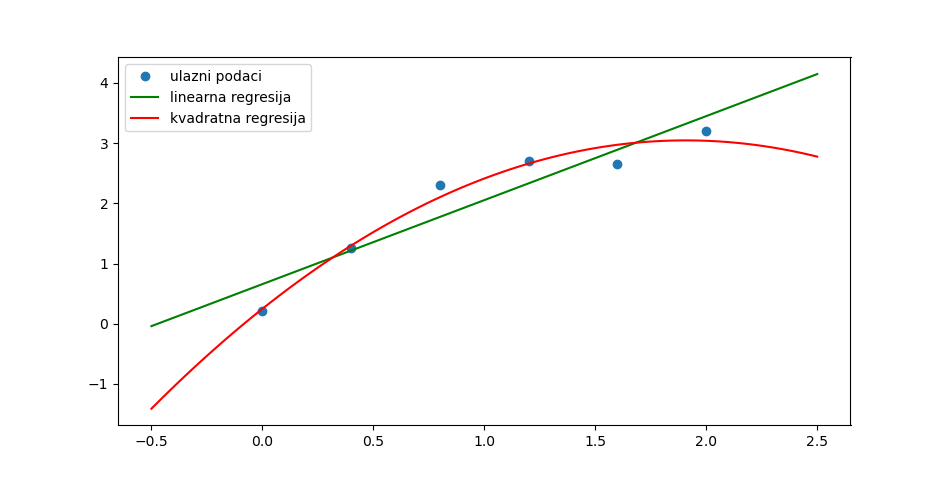
\includegraphics[width=\linewidth]{fig/regresija.png}
